\documentclass[12pt]{article}

\usepackage[margin=1in]{geometry}
\usepackage{amsmath, amssymb, amsthm, amsfonts}
\usepackage{tikz}
\usepackage{hyperref}
\usepackage{url}

% ------------------------------------------------------------
% Theorem Environments
% ------------------------------------------------------------
\theoremstyle{plain}
\newtheorem{theorem}{Theorem}[section]
\newtheorem{lemma}[theorem]{Lemma}
\newtheorem{proposition}[theorem]{Proposition}
\newtheorem{corollary}[theorem]{Corollary}

\theoremstyle{definition}
\newtheorem{definition}[theorem]{Definition}
\newtheorem{example}[theorem]{Example}
\newtheorem{remark}[theorem]{Remark}

% ------------------------------------------------------------
% Title and Author
% ------------------------------------------------------------
\title{\textbf{Unification of Linguistics Through a Generalized Theory of\\
the Universal Linguistic Functor (ULF)}}
\author{
  \textbf{Matthew Long}\\
  \textit{Magneton Labs}
}
\date{\today}

\begin{document}
\maketitle

\begin{abstract}
We present a generalized theory of the Universal Linguistic Functor (ULF) that aims to unify core principles of syntax, semantics, and cross-linguistic variation under a category-theoretic framework. We develop the concept of a universal grammar object as an initial object in the category of grammars, extend this to presheaves capturing language-specific parameters, and show how enriched category structures and topos theory can yield a graded and context-sensitive semantics. Proof sketches of key propositions and theorems are provided to elucidate the mathematical basis of our framework. Potential applications to natural language processing (NLP) and cognitive modeling underscore the practical value of a unifying category-theoretic approach to linguistic theory.
\end{abstract}

\tableofcontents

\section{Introduction}\label{sec:intro}
The quest for a unifying theory of language has motivated generations of linguists, mathematicians, and computer scientists. The advent of formal language theory, type-theoretic grammars, and category-theoretic semantics has offered partial solutions, but each discipline often proceeds with separate assumptions and methods. In this paper, we aim to bridge these approaches through a \emph{generalized} Universal Linguistic Functor (\textbf{ULF}) framework.

Building upon earlier versions of ULF \cite{Lewis}, we propose three key features:
\begin{enumerate}
    \item \textbf{Universal Grammar as an Initial Object.} We treat universal grammar as an initial object \(\mathcal{U}\) in the category \(\mathbf{Gram}\) of formal grammars. This encodes the property that every individual grammar factors uniquely from a universal blueprint.
    \item \textbf{Presheaf-based Variation.} To model cross-linguistic diversity, we introduce presheaves over a category of linguistic settings (e.g., morphological or syntactic parameters). This captures how languages systematically vary while preserving core structural constraints.
    \item \textbf{Enriched \& Topos-Theoretic Semantics.} We augment Boolean semantics with enrichment over \([0,1]\) to capture gradience and fuzziness. Further, a topos-theoretic perspective accommodates intensionality, modality, and other context-dependent phenomena.
\end{enumerate}

We provide proof sketches for key theorems—most notably, the existence of a universal grammar object, which parallels free constructions in algebraic settings, and the commutativity of certain presheaf diagrams ensuring consistency across linguistic variations. We conclude with applications in computational linguistics and potential avenues for future research.

\section{Background and Motivation}
\subsection{Category Theory in Linguistics}
Category theory offers a powerful language of objects (linguistic categories) and morphisms (structure-preserving maps) that has been leveraged in formal semantics \cite{Montague}, syntax-semantics interface \cite{BarkerShan}, and beyond.  

\begin{definition}[Category]
A \emph{category} \(\mathbf{C}\) consists of a collection of objects and a collection of morphisms between these objects, satisfying composition and identity axioms. 
\end{definition}

In syntax, objects can be \emph{syntactic categories} (e.g., noun phrase, verb phrase), and morphisms can represent \emph{derivational} or \emph{projection} operations. In semantics, objects may be \emph{semantic types}, and morphisms encode \emph{meaning transformations}.

\subsection{Functors and Natural Transformations}
A \emph{functor} \(F: \mathbf{C} \to \mathbf{D}\) transports the structure of one category \(\mathbf{C}\) into another \(\mathbf{D}\). In linguistic theory, a functor often maps syntactic constructs to semantic interpretations. Natural transformations capture systematic ways to modify or interpret these functorial mappings.

\subsection{Topos Theory}
\emph{Topos} theory generalizes set theory with richer internal logics, enabling the modeling of intensionality, context dependence, and possibly dynamic semantics \cite{LambekScott}. A topos can be thought of as a category that behaves like \(\mathbf{Set}\) but admits more general subobject classifiers and internal languages, crucial for capturing certain linguistic phenomena.

\section{The Category of Grammars \(\mathbf{Gram}\)}
We begin by defining the category \(\mathbf{Gram}\), whose objects are \emph{formal grammars} and whose morphisms preserve grammatical structure.

\begin{definition}[Formal Grammar]
A \emph{formal grammar} \(G\) is a 4-tuple \((N, \Sigma, P, S)\), or an equivalent generative mechanism, specifying a set of \emph{nonterminal} symbols \(N\), \emph{terminal} symbols \(\Sigma\), a set \(P\) of production rules or constraints, and a start symbol \(S\). For more sophisticated frameworks (e.g., Minimalist Grammars), the set of operations is more elaborate but can still be packaged formally.
\end{definition}

\begin{definition}[Morphisms in \(\mathbf{Gram}\)]
A morphism \(\phi: G_1 \to G_2\) in \(\mathbf{Gram}\) is a \emph{structure-preserving map} such that:
\begin{enumerate}
    \item Nonterminals in \(G_1\) map to compatible nonterminals (or categories) in \(G_2\).
    \item Production rules in \(G_1\) are sent to valid derivations or constraints in \(G_2\).
    \item If \(G_1\) has a start symbol \(S_1\), it must map to a valid start symbol \(S_2\) or an equivalent initial category in \(G_2\).
\end{enumerate}
\end{definition}

\subsection{Universal Grammar as Initial Object}
One major postulate in ULF is the existence of a \emph{universal grammar object} \(\mathcal{U}\) in \(\mathbf{Gram}\). Recall that:

\begin{definition}[Initial Object]
An object \(I\) in a category \(\mathbf{C}\) is \emph{initial} if for every object \(C \in \mathbf{C}\) there is a unique morphism \(I \to C\).
\end{definition}

Translating this to our context:

\begin{theorem}[Existence of a Universal Grammar Object]\label{thm:UG}
Suppose there is a set of universal features, principles, and constraints from which all particular grammars can be obtained uniquely by specifying language-particular parameter settings. Then there exists an object \(\mathcal{U} \in \mathbf{Gram}\) that is initial.
\end{theorem}

\begin{proof}[Proof Sketch]
\ 
\begin{enumerate}
    \item \textbf{Constructing a Candidate \(\mathcal{U}\).} Start with a “free grammar” over the universal feature set. This includes minimal syntactic categories and constraints hypothesized to be universal across languages.
    \item \textbf{Uniqueness of Morphisms.} For any grammar \(G\), interpret each universal feature or principle from \(\mathcal{U}\) into the corresponding elements of \(G\). By the universal property of free constructions, the morphism is forced, ensuring uniqueness.
    \item \textbf{Closure under Parameterization.} Any parameter not fixed in \(\mathcal{U}\) is specialized when mapping into a particular grammar \(G\). This is consistent with generative linguistic theories that specify how \(\mathcal{U}\) can yield all \emph{possible} human grammars.
\end{enumerate}
Thus, \(\mathcal{U}\) satisfies the definition of an initial object in \(\mathbf{Gram}\).
\end{proof}

\section{Presheaf-based Variation}
\subsection{Modeling Parameters and Contexts}
While Theorem \ref{thm:UG} captures universal principles, \emph{language variation} demands a mechanism to track differences in morphological, phonological, and typological features. We let \(\mathbf{Lin}\) be the category of \emph{linguistic contexts}, where objects are parameter configurations (e.g., whether a language is pro-drop, whether it has SVO or SOV order, etc.), and morphisms represent transitions between these configurations.

\begin{definition}[Presheaf]
A \emph{presheaf} \(P\) on a category \(\mathbf{C}\) is a functor \(P : \mathbf{C}^{op} \to \mathbf{Set}\).
\end{definition}

Hence, we define:

\begin{definition}[Language Variation Presheaf]
A presheaf \(P: \mathbf{Lin}^{op} \to \mathbf{Set}\) assigns to each linguistic context \(L\) a set \(P(L)\) of possible \emph{grammatical realizations} (or derivations, or lexical expansions), and to each morphism \(L_1 \to L_2\) in \(\mathbf{Lin}\) (e.g., adjusting a parameter) a restriction map \(P(L_2) \to P(L_1)\).
\end{definition}

\subsection{Commutativity of Variation Diagrams}
Often, multiple linguistic modules (syntax, phonology, morphology) must remain consistent. If \(P\) and \(Q\) are presheaves corresponding to different modules, we want them to “commute” in certain diagrammatic senses (e.g., combining morphological and syntactic transformations yields consistent outputs).

\begin{theorem}[Presheaf Commutativity]\label{thm:Comm}
Let \(P, Q: \mathbf{Lin}^{op} \to \mathbf{Set}\) be presheaves modeling different linguistic modules. Suppose there is a natural transformation \(\alpha: P \to Q\) capturing how syntactic forms map into morphological forms. Then the relevant diagrams in \(\mathbf{Lin}^{op}\) commute under composition, ensuring global consistency of the two modules.
\end{theorem}

\begin{proof}[Proof Sketch]
By the definition of a natural transformation, for every morphism \(\sigma: L_2 \to L_1\) in \(\mathbf{Lin}\), we have a commutative square ensuring \(\alpha\) intertwines with the presheaf restriction maps. This square-commutativity then extends by composition, giving a larger commuting diagram across all relevant contexts.
\end{proof}

The result ensures that if morphological modifications follow from syntactic ones in a uniform, natural-transformational way, no contradiction arises across the entire parameter space.

\section{Enriched and Topos-Theoretic Semantics}
\subsection{Enrichment Over \([0,1]\)}
In classical Montague-style semantics, interpretations are Boolean. However, linguistic phenomena such as gradable adjectives (“tall,” “fast,” “heavy”) and prototype effects (“robin” is more typical of “bird” than “penguin”) suggest a graded notion of meaning. We capture this with an \emph{enriched category}:

\begin{definition}[Enriched Category]
A category \(\mathbf{C}\) is \emph{enriched} over a monoidal category \(\mathbf{V}\) if instead of hom-sets \(\mathbf{C}(A,B)\), we have objects in \(\mathbf{V}\), and composition is given via \(\mathbf{V}\)-morphisms that respect the monoidal structure.
\end{definition}

Taking \(\mathbf{V}\) as \(([0,1], \times, 1)\), morphisms in our semantic category can be degrees (ranging in \([0,1]\)) of applicability or truth. This allows:

\begin{itemize}
    \item Gradience in category membership.
    \item Partial truth for vague predicates.
    \item Weighted or probabilistic semantic interpretations.
\end{itemize}

\subsection{Topos-Theoretic Considerations}
A \emph{Grothendieck topos} \(\mathbf{E}\) can serve as a more general environment for semantics, where sets of linguistic entities might vary according to contexts or possible worlds. Internal logic within \(\mathbf{E}\) can handle intensional phenomena such as modality (\(\Box, \Diamond\)) or hidden parameters. If \(\mathbf{Lin}\) is treated as a \emph{site}, we can build a topos of sheaves (or presheaves with additional gluing conditions) capturing how meaning is compiled across local contexts.

\section{Proof Sketches for Key Theorems}
\subsection{Universal Grammar Object}
We revisit Theorem \ref{thm:UG}, focusing on the notion of universal features and how they might be systematically extended to any particular grammar. The technical details rely on standard free-object constructions in category theory:

\begin{enumerate}
    \item \textbf{Free Grammar Generation.} Define a set \(F\) of universal linguistic features (Merge, Move, case assignment, etc.) plus constraints (e.g., locality constraints). A free construction yields the largest grammar with no additional idiosyncratic features. 
    \item \textbf{Well-Formed Mappings.} For any particular grammar \(G\), there is a unique grammar homomorphism from the free grammar to \(G\), which interprets or “assigns values” to each universal principle.
    \item \textbf{Initiality Criterion.} The universal grammar \(\mathcal{U}\) is the unique (up to isomorphism) object from which these unique homomorphisms emanate, completing the initial-object definition.
\end{enumerate}

\subsection{Presheaf Commutativity}
Theorem \ref{thm:Comm} states that natural transformations between presheaves yield commutative diagrams across contexts in \(\mathbf{Lin}\). The key ingredient is the definition of a natural transformation:

\[
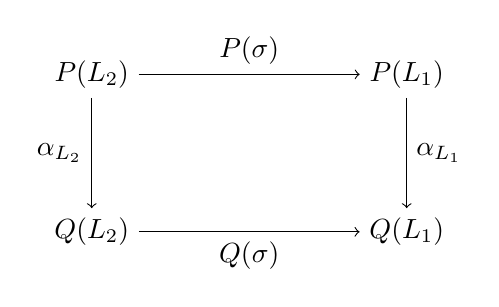
\begin{tikzpicture}[node distance=4em, auto]
  \node (L2) at (0,0) {$P(L_2)$};
  \node (L1) at (4,0) {$P(L_1)$};
  \node (L2Q) at (0,-2) {$Q(L_2)$};
  \node (L1Q) at (4,-2) {$Q(L_1)$};

  \draw[->] (L2) to node {$P(\sigma)$} (L1);
  \draw[->] (L2Q) to node [below] {$Q(\sigma)$} (L1Q);
  \draw[->] (L2) to node [left] {$\alpha_{L_2}$} (L2Q);
  \draw[->] (L1) to node [right] {$\alpha_{L_1}$} (L1Q);
\end{tikzpicture}
\]

This “square” must commute for every \(\sigma: L_2 \to L_1\). The composition property extends to all sequences of morphisms in \(\mathbf{Lin}\), guaranteeing global consistency.

\section{Applications}
\subsection{Natural Language Processing (NLP)}
\begin{itemize}
    \item \textbf{Structure-Preserving Translation.} Functorial mappings between grammars can guide machine translation systems to respect morphological, syntactic, and semantic structure. 
    \item \textbf{Parameter Discovery.} The presheaf approach suggests that discovering or learning morphological/phonological parameters can be seen as searching for consistent “fiber” structures in a presheaf. 
    \item \textbf{Hybrid Symbolic-Statistical Models.} By coupling ULF’s formal backbone with neural embeddings, one could combine interpretability with data-driven performance.
\end{itemize}

\subsection{Cognitive and Psycholinguistic Modeling}
\begin{itemize}
    \item \textbf{Prototype Semantics.} Enriched categories allow a graded notion of membership, aligning with prototype or exemplar theories in cognitive semantics.
    \item \textbf{Ambiguity and Monads.} A monadic approach (commonly used in functional programming) can capture how language users maintain sets of possible interpretations, resolving them contextually.
    \item \textbf{Dynamic Semantics.} Topos-theoretic internal languages can encode updates to discourse contexts, bridging dynamic semantics with a categorical perspective.
\end{itemize}

\section{Future Directions and Open Problems}
\subsection{Integration with Type Theory}
Type-theoretic grammars, especially those used in proof assistants (Coq, Agda), share structural parallels with categorical semantics. Developing translations of ULF into typed functional languages could yield:
\begin{itemize}
    \item Verified grammars in proof assistants.
    \item Deep synergy between syntax, semantics, and type-checking.
\end{itemize}

\subsection{Further Enrichment}
One could consider multi-dimensional or topological enrichments to model more nuanced phenomena (e.g., conceptual space geometry, as in \cite{Gardenfors}). This might capture aspects like distance in semantic space or continuous changes across registers and dialects.

\subsection{Computational Feasibility}
Applying the full machinery of presheaves and toposes at scale is challenging. Further research on:
\begin{itemize}
    \item Efficient representations of presheaves (e.g., via hierarchical or neural compressions).
    \item Partial or approximate functorial translations for large-scale corpora.
\end{itemize}

\section{Conclusion}
This paper has presented a generalized theory of the Universal Linguistic Functor framework, harnessing category theory to unify linguistic phenomena from syntactic derivations to semantic interpretations and cross-linguistic variation. By positioning universal grammar as an initial object, employing presheaves to handle the parameter space of languages, and incorporating enriched or topos-theoretic semantics, ULF establishes a robust yet flexible architecture. Our proof sketches highlight the internal consistency and mathematical rigor of this approach.

From computational linguistics to cognitive science, the potential applications are vast. Symbolic and neural methods alike can profit from the structural insights of category theory, with the possibility of new, interpretable, and mathematically grounded NLP systems. Future work will determine the deeper ramifications of adopting ULF as a central organizing principle for linguistic theory.

\subsection*{Acknowledgments}
The author gratefully acknowledges discussions with colleagues in linguistics, computer science, and category theory who have influenced this work. Any errors are the responsibility of the author alone.

\begin{thebibliography}{99}

\bibitem{Lewis}
Lewis, D. (1970). ``General Semantics.'' \textit{Synthese}, 22, 18--67.

\bibitem{Montague}
Montague, R. (1974). \textit{Formal Philosophy}. Yale University Press.

\bibitem{BarkerShan}
Barker, C., \& Shan, C. (2014). \textit{Continuations and Natural Language}. Oxford University Press.

\bibitem{LambekScott}
Lambek, J., \& Scott, P. (1986). \textit{Introduction to Higher-Order Categorical Logic}. Cambridge University Press.

\bibitem{Gardenfors}
G\"{a}rdenfors, P. (2000). \textit{Conceptual Spaces: The Geometry of Thought}. MIT Press.

\end{thebibliography}

\end{document}
